\section{Method}


% 0114
\textbf{Overview.} 
To solve the obstacles identified above, we present Z-Erase. First, we introduce the \emph{Stream Disentangled Concept Erasure Framework} for single-stream models. This structural mechanism provides a safe subspace for our erasure and preservation losses, and enables previous erasure methods to function effectively in the single-stream setting. Second, to handle the delicate trade-off between erasure and preservation, we propose a \emph{Lagrangian-Guided Adaptive Erasure Modulation} algorithm based on this framework. Instead of using fixed weights, this novel algorithm dynamically adjusts erasure strength to strictly guarantee utility. Together, these two key parts make stable and effective erasure possible on single-stream models. Next, we introduce each in detail.





% 0114
\subsection{Stream Disentangled Concept Erasure Framework}

As analyzed in Section~\ref{sec:motivation}, the core challenge in single-stream models is the strict coupling of text and image processing: directly fine-tuning shared weights to erase a text concept will unavoidably distort the visual signal, causing generation collapse. To resolve this architectural bottleneck, we propose the \emph{Stream Disentangled Concept Erasure Framework}, which is designed to structurally isolate the parameter update trajectory.

Specifically, we first control which modality receives updates. Let $\mathbf{S}_T = \mathtt{diag}(\mathbf{0}_{n_I}, \mathbf{I}_{n_T}) \in \mathbb{R}^{(n_I + n_T) \times (n_I + n_T)}$ be a token-wise selection operator that acts as a binary gate. This operator assigns zeros to image tokens and ones to text tokens, creating a physical barrier that restricts low-rank updates $\Delta \mathbf{W}$ exclusively to textual hidden states while bypassing the visual stream.


Formally, we apply this gating to the linear projection layers. For weights $\mathbf{W} \in \{\mathbf{W}_Q, \mathbf{W}_K, \mathbf{W}_V\}$, the modified forward pass is defined as $\mathbf{H}' = \mathbf{H} \mathbf{W} + \mathbf{S}_T \mathbf{H} (\Delta \mathbf{W})$. By factoring the hidden states $\mathbf{H}$ into visual and textual segments, this yields a clean separation in the adaptation dynamics:
\begin{equation}
\begin{aligned}
\begin{bmatrix} \mathbf{H}_{img}' \\ \mathbf{H}_{txt}' \end{bmatrix}
=
\begin{bmatrix} \mathbf{H}_{img} \\ \mathbf{H}_{txt} \end{bmatrix}
\begin{bmatrix}
\underbrace{\mathbf{W}}_{\text{Frozen}} 
& \raisebox{-5pt}{$\mathbf{O}$}\\[2pt]
\raisebox{-5pt}{$\mathbf{O}$}
& \underbrace{\mathbf{W} + \Delta \mathbf{W}}_{\text{Trainable, Concept Erasure}}
\end{bmatrix}.
\end{aligned}
\label{eq: Stream Disentangled Concept Erasure Framework}
\end{equation}
This design constructs a safe optimization subspace for concept erasure in single-stream models. The key idea is to restrict gradient updates to the textual hidden states $\mathbf{H}_{txt}$ while keeping the pixel-generation backbone $\mathbf{H}_{img}$ frozen. This isolation is critical, because the projection weights jointly govern both semantic understanding and image synthesis. Without such decoupling, erasure gradients inevitably perturb the shared attention pathways and cause the generation collapse observed in naive fine-tuning. With this subspace in place, previous erasure methods become operational again in the unified single-stream architecture.




Within this safe subspace, we implement concept erasure as an adversarial fine-tuning process. Our goal is to suppress a target concept set $\mathcal{D}_{er}$, while anchoring the model on an unrelated concept set $\mathcal{D}_{pr}$ to ensure general utility remains unaffected. The two objects are defined as:


\textbf{Erasure objective.}
Motivated by the negative guidance idea introduced by ESD~\cite{esd}, we start from direct trajectory intervention in flow matching. The first sub-loss in our Z-Erase aims to suppress the visual manifestation of the target concept during the denoising trajectory. Specifically, the erase loss is defined as:
\begin{equation}
\label{eq: L erase}
\begin{aligned}
&\mathcal{L}_{erase} 
     = \mathbb{E}_{x_t, t, c_{er}\sim\mathcal{D}_{er}} \Big\| v_{\theta+\Delta\theta}(x_t,c_{er},t) - \\
    & \big[ v_{\theta}(x_t, \varnothing, t) -\eta\big(v_{\theta}(x_t,c_{er},t)-v_{\theta}(x_t, \varnothing, t)\big) \big] \Big\|_2^2.
\end{aligned}
\end{equation}
Here, $\eta$ is the negative guidance factor and directly influences how aggressively the concept is erased. $\theta$ denotes the pretrained model parameters and $\Delta\theta$ is the learnable LoRA weights for erasure. $x_t$ denotes the latent at timestep $t$, starting from random noise $x_T$ where $T$ is the total timesteps. $v_{\theta}(x_t, \varnothing, t)$ corresponds to the unconditional velocity prediction (with empty prompt), while $c_{er} \in \mathcal{D}_{er}$ identifies the concept to erase. In flow matching, $v$ represents the velocity field guiding the trajectory between distributions, which makes it a natural site for concept-level intervention.

Furthermore, building on the \emph{single-stream attention} insights discussed in Section~\ref{sec:motivation}, we further reduce the influence of the erased concept by suppressing the attention assigned to its localized keywords:
\begin{equation}
\label{eq: L attn}
    \mathcal{L}_{attn} = \sum_{idx = start}^{end} \textbf{A}_{attn}[:,:,idx],
\end{equation}
To avoid overfitting to fixed token positions, we also randomly shuffle the word order during training, keeping the index range dynamic while preserving the original meaning.

Together, these two terms form the erasure objective:
\begin{equation}
    \mathcal{L}_{er} = \mathcal{L}_{erase} + \mathcal{L}_{attn}.
\end{equation}




\begin{figure}[t]
	\centering
	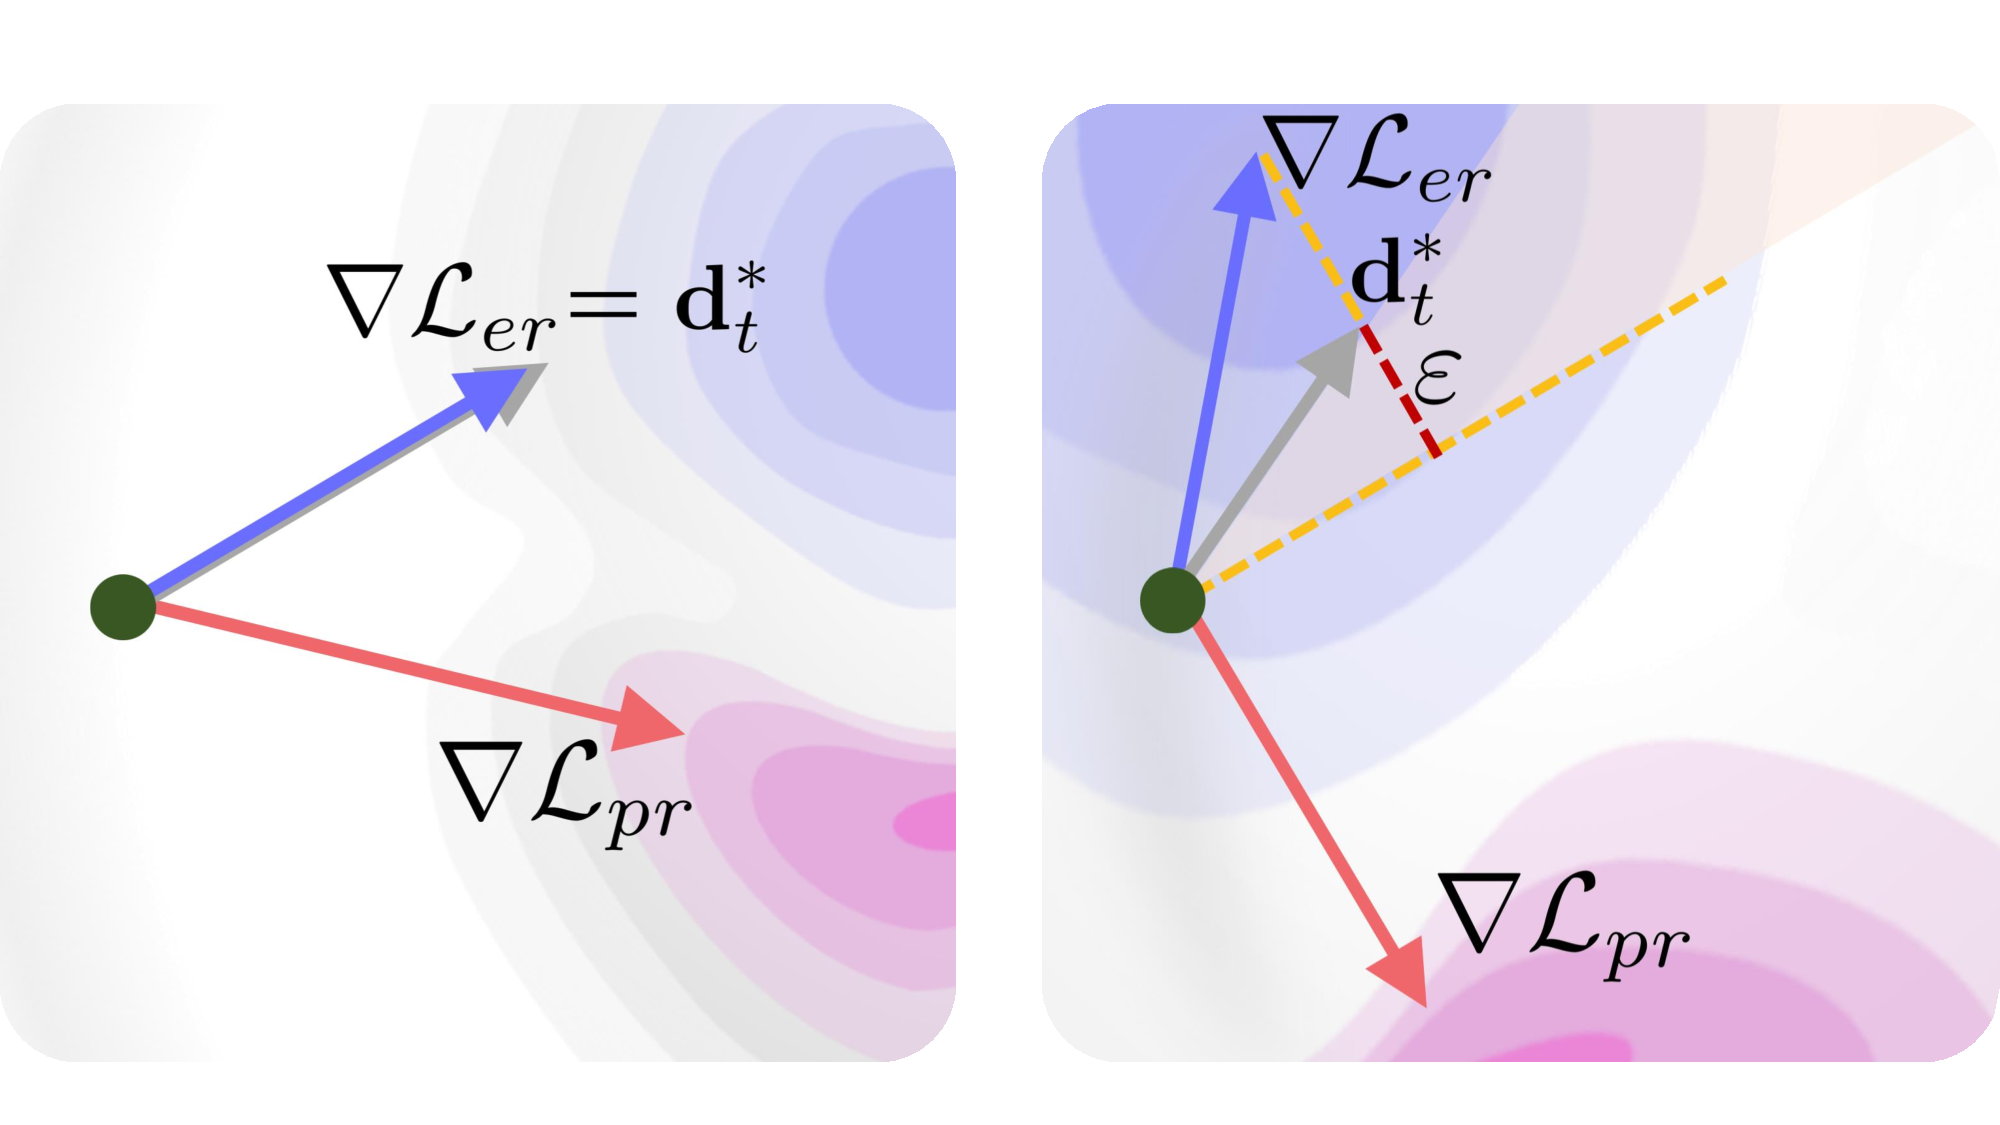
\includegraphics[width=0.67\linewidth]{fig/balance_optimization.pdf}
    \caption{\textbf{Dynamic balancing of erasure and preservation gradients.} \textit{Left:} When $\nabla \mathcal{L}_{er}$ does not conflict with $\nabla \mathcal{L}_{pr}$, the erasure gradient itself is the update direction. \textit{Right:} When the gradients conflict, the update direction $\mathbf{d}^*_t$ is obtained by steering $\nabla \mathcal{L}_{er}$ toward $\nabla \mathcal{L}_{pr}$ until the preservation constraint $\varepsilon$ is satisfied.}
    \label{fig:balance_optimization}
    \vspace{-10pt}
\end{figure}



\textbf{Preservation objective.}
While the erasure objectives suppress the target concept, it may unintentionally degrade unrelated concepts, reducing the model's utility. For example, given the prompt \textit{``A nude girl"}, our goal is to erase $c_{er}$ \textit{``nude"} while ensuring the model can still generate images of an unrelated concept $c_{pr} \in \mathcal{D}_{pr}$ normally, \textit{e.g.,} girl. To preserve usability, we constrain the shift in the generation process for concepts that should remain untouched:
\begin{equation}
\label{eq: L pr}
\begin{aligned}
&\mathcal{L}_{pr}
= \mathbb{E}_{x_t,t}
    \Big\|
        v_{\theta + \Delta \theta}(x_t, \varnothing, t)
        - v_{\theta}(x_t, \varnothing, t)
    \Big\|_2^2 + \\
&  \mathbb{E}_{x_t,t,\;c_{pr}\sim\mathcal{D}_{pr}}
    \Big\|
        v_{\theta + \Delta \theta}(x_t,c_{pr},t)
        - v_{\theta}(x_t,c_{pr},t)
    \Big\|_2^2 .
\end{aligned}
\end{equation}

Finally, combining the erasure term, attention suppression, and preservation constraint completes the set of learning objectives for Z-Erase.

%0116
\subsection{Lagrangian-Guided Adaptive Erasure Modulation}
\label{section: Constraint-Aware Dynamic Balancing}

With our erasure and preservation objectives in place, the remaining challenge is how to optimize them together. Existing methods typically adopt linear scalarization (\textit{e.g.}, MACE) or multi-objective optimization (\textit{e.g.}, EraseAnything). However, simply combining erasure and preservation objectives that have inherent conflict fails to find a balanced solution, as proved in multitask learning literature~\cite{hu2024revisiting}. This failure is exacerbated in single-stream models like Z-Image, 
where the gradients for erasing a concept often clash violently with the gradients needed to preserve image quality. Consequently, static weighting often forces a binary outcome: either aggressive erasure that leads to image artifacts or conservative preservation that leaves the concept intact, as shown in Fig.~\ref{fig:main_cmp}.







\begin{algorithm}[t]
   \caption{Training Procedure of Z-Erase}
   \label{alg:z-erase}
\begin{algorithmic}
   \STATE {\bfseries Input:} Pretrained model $\theta_0$, erasure concept set $\mathcal{D}_{er}$, preservation concept set $\mathcal{D}_{pr}$, total iteration steps $M$.
   \STATE {\bfseries Hyperparameters:} Learning rates $\alpha$ (for model), $\beta$ (for $\lambda$), tolerance $\varepsilon$, initial $\lambda_0 = 0$.
   
   \FOR{iteration $t=1$ {\bfseries to} $M$}
       \STATE \textbf{\ding{182}} Calculate preservation loss change:
       \STATE \quad $\tilde{g}_t = \frac{1}{\alpha} (\mathcal{L}_{pr}(\theta_{t-1}) - \mathcal{L}_{pr}(\theta_{t})) + \varepsilon$.
       \STATE \textbf{\ding{183}} Update constraint weight: $\lambda_{t+1} \leftarrow \lambda_t - \beta \tilde{g}_t$.
       \STATE \textbf{\ding{184}} Sample batches $c_{er} \sim \mathcal{D}_{er}$ and $c_{pr} \sim \mathcal{D}_{pr}$.
       \STATE \textbf{\ding{185}} Compute losses $\mathcal{L}_{er}$ and $\mathcal{L}_{pr}$ with Eq.~\ref{eq: L erase} to \ref{eq: L pr}.
       \STATE \textbf{\ding{186}} Compute total balanced objective:
       \STATE \quad $\mathcal{L}_{total} = \mathcal{L}_{er} + \lambda_{t+1} \mathcal{L}_{pr}$
       \STATE \textbf{\ding{187}} Update LoRA weights:
       \STATE \quad $\Delta \theta_{t+1} \leftarrow \Delta \theta_t - \alpha \nabla_{\Delta \theta} \mathcal{L}_{total}$
   \ENDFOR
   \STATE {\bfseries Output:} Final erased model $\theta' = \theta_0 + \mathbf{S}_T(\Delta \theta_M)$
\end{algorithmic}
\end{algorithm}



To resolve this dilemma, we further introduce a \emph{Lagrangian-Guided Adaptive Erasure Modulation} algorithm. Unlike static weighting that struggles to find a stable balance, we treat erasure and preservation as a dynamic constrained optimization problem. The goal is to converge to a controllable point on the Pareto front~\cite{yu2020gradientsurgerymultitasklearning}, where erasure cannot be further improved without sacrificing preservation. 
Specifically, we increase erasure under a preservation tolerance. At training step $t$ with parameters $\theta_t$, we solve for an update direction $\mathbf{d}_t$ that maximizes the descent of the erasure objective $\mathcal{L}_{er}$ while constraining the increase of $\mathcal{L}_{pr}$ to remain within a small tolerance $\varepsilon$:
\begin{equation}
\label{eq: our goal}
    \max_{\mathbf{d}_t} \nabla \mathcal{L}_{er}(\theta_t) \cdot \mathbf{d}_t - \frac{1}{2}\|\mathbf{d}_t\|^2 
    , \,\,
    \text{s.t.} \nabla \mathcal{L}_{pr}(\theta_t) \cdot \mathbf{d}_t \ge -\varepsilon,
\end{equation}
where $\|\mathbf{d}_t\|^2$ is the regularization to avoid unbounded solutions. By introducing a Lagrange multiplier $\lambda_t \ge 0$, we can rewrite this as a dual problem:
\begin{equation}
\label{eq: dual problem}
    \min_{\lambda_t \ge 0} \mathcal{L}_{t}(\lambda_t) =  \frac12 \big\| \nabla \mathcal L_{er}(\theta_t) + \lambda_t \nabla \mathcal L_{pr}(\theta_t) \big\|^2 + \lambda_t \varepsilon.
\end{equation}
% This formulation shifts the optimization to solving for a  dynamic weight $\lambda_t$ that satisfies the constraint. With this dual variable $\lambda_t$ defined, differentiation \textit{w.r.t.} $\mathbf{d}_t$ yields a closed-form solution for the optimal update direction $\mathbf{d}^*_t$, which takes the form of \emph{gradient surgery}:
This formulation shifts the optimization into finding a dynamic dual weight $\lambda_t$ that satisfies the constraint. By determining the optimal $\lambda_t$ and minimizing the Lagrangian \textit{w.r.t.} $\mathbf{d}_t$, we derive a closed-form solution $\mathbf{d}^*_t$ that naturally takes the form of \emph{gradient surgery}:
\begin{equation}
\label{eq: dt closed-form solution}
    \mathbf{d}^*_t = \begin{cases} 
\nabla \mathcal{L}_{er}(\theta_t) + \lambda^*_t \nabla \mathcal{L}_{pr}(\theta_t), & \text{if } \text{conflict exists} (\lambda_t^* > 0) \\
\nabla \mathcal{L}_{er}(\theta_t), & \text{otherwise}
\end{cases}
\end{equation}
where
\begin{equation}
\label{eq: lambda_t closed-form solution}
    \lambda_t^* = \frac{-\nabla\mathcal{L}_{er}(\theta_t) \cdot \nabla \mathcal{L}_{pr}(\theta_t) - \varepsilon}{\left\|\nabla \mathcal{L}_{pr}(\theta_t)\right\|^2}.
\end{equation}
Due to space limit, we provide full derivation from Eq.~\ref{eq: our goal} to Eq.~\ref{eq: lambda_t closed-form solution} in Appendix~\ref{appendix: Derivation of the dual problem} and ~\ref{appendix: Derivation of the closed-form solution for the optimal direction}. Here, $\lambda^*_t$ acts as a dynamic gatekeeper. If the erasure gradient attempts to hurt preservation capability beyond $\varepsilon$, $\lambda^*_t$ becomes positive, effectively projecting the update onto a safe subspace, as illustrated in Fig.~\ref{fig:balance_optimization}.



\begin{figure}[t]
	\centering
	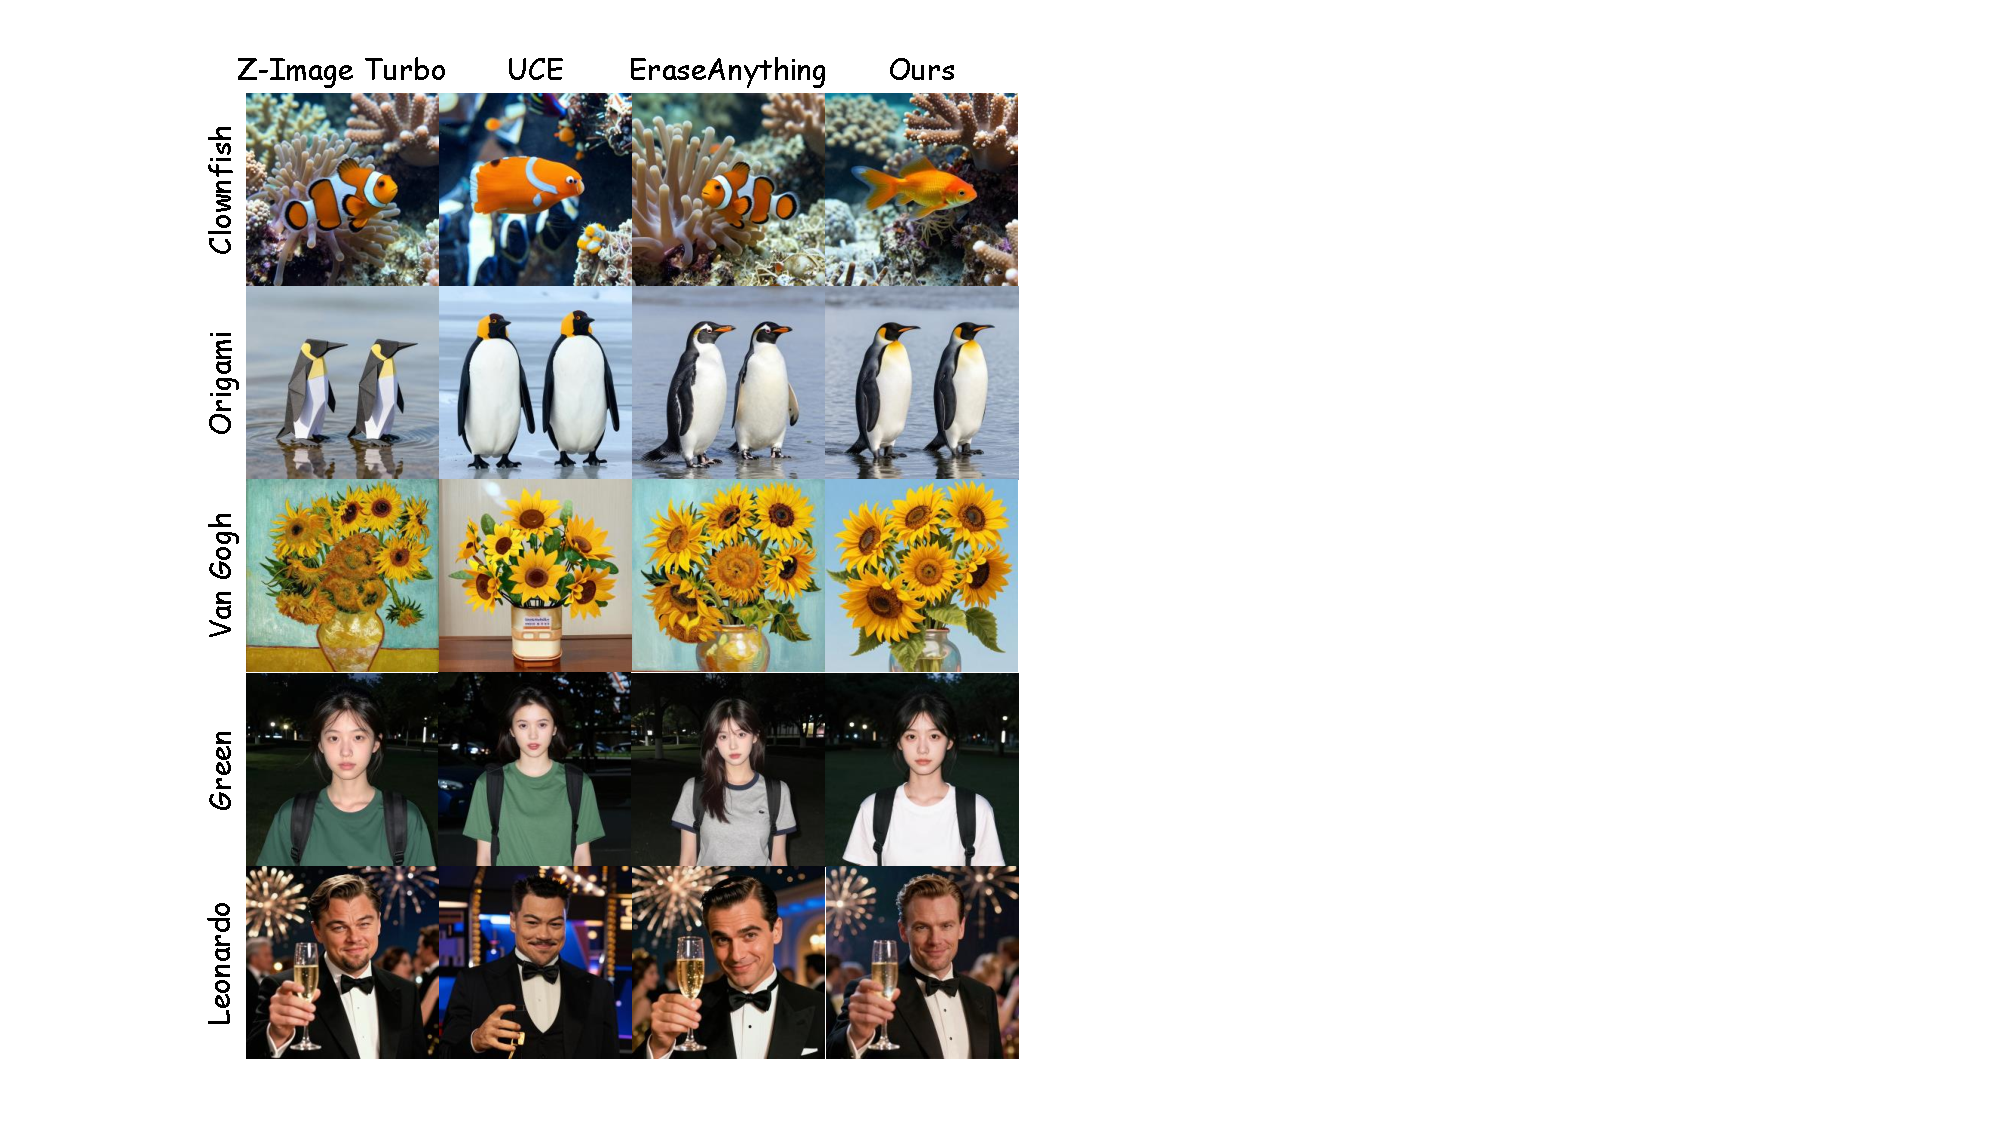
\includegraphics[width=0.8\linewidth]{fig/main_cmp.pdf}
    \caption{\textbf{Single-concept erasure.} Our method removes both concrete and abstract concepts while preserving image quality with minimal collateral changes. In contrast, UCE severely distorts images and introduces strong artifacts, whereas EraseAnything may fail to erase or causes noticeable semantic shifts.}
    \label{fig:main_cmp}
    \vspace{-5pt}
\end{figure}



However, we find that explicitly computing $\lambda_t^*$ requires two independent backward passes to obtain $\nabla \mathcal{L}_{er}$ and $\nabla \mathcal{L}_{pr}$, doubling the training cost. To make this theoretically grounded approach computationally feasible, we employ an implicit approximation key to our adaptive modulation. 
Specifically, instead of directly solving for the exact $\lambda_t$ at every step, we approximate the minimum of the dual problem Eq.~\ref{eq: dual problem} by iteratively updating $\lambda_t$ via gradient descent:
\begin{equation}
% \vspace{-5pt}
\label{eq: iteratively update lambda t via gradient descent approximation}
    \lambda_{t+1} = \lambda_t - \beta \nabla_{\lambda_{t}} \mathcal{L}_{t}(\lambda_t),
% \vspace{-5pt}
\end{equation}
where $\beta$ controls the sensitivity of the weight adjustment. However, calculating $\nabla_{\lambda_{t}} \mathcal{L}_{t}$ still needs the gradient $\nabla \mathcal{L}_{pr} \cdot \mathbf{d}_t$, which brings us back to the original computational bottleneck. To resolve this, we approximate this dot product $\nabla \mathcal{L}_{pr} \cdot \mathbf{d}_t$ using the first-order Taylor expansion: 
\begin{align}
\nabla_{\lambda_{t}} \mathcal{L}_{t}(\lambda_t) & = \nabla \mathcal{L}_{pr}(\theta_t) \cdot (\nabla \mathcal{L}_{er}(\theta_t) + \lambda_t \nabla \mathcal{L}_{pr}(\theta_t)) + \varepsilon \nonumber \\
& = \nabla \mathcal{L}_{pr}(\theta_t) \cdot \mathbf{d}_t + \varepsilon \nonumber \\
& \approx \frac{1}{\alpha} \left( \mathcal{L}_{pr}(\theta_t) - \mathcal{L}_{pr}(\theta_{t+1}) \right) + \varepsilon. \label{first-order Taylor expansion}
\end{align}
Here, $\alpha$ is the learning rate of the model. This step is crucial: it translates the expensive geometric projection (dot product of gradients) into a cheap scalar observation (change in loss values). As a result, we obtain an approximate method for solving $\lambda_t$ without extra backpropagation:
\begin{equation}
    \lambda_{t+1} = \lambda_t - \beta \tilde{g}_t, \,\, \text{where } \tilde{g}_t = \frac{1}{\alpha} \left( \mathcal{L}_{pr}(\theta_{t-1}) - \mathcal{L}_{pr}(\theta_{t}) \right) + \varepsilon.
\end{equation}
This creates a self-regulating loop: if the model violates the preservation constraint (\textit{i.e.}, $\mathcal{L}_{pr}$ increases significantly such that $\tilde{g}_t < 0$), $\lambda$ increases, forcing the model to prioritize preservation in the next unified backward pass; otherwise, $\lambda$ decays, allowing aggressive concept erasure.






Notably, a major advantage of this algorithm is that it provides a theoretical bound on how much the model's original capabilities will shift. We can prove the degradation of the preservation capability is bounded by:
\begin{equation}
\label{eq: Lpr is bounded by}
    \mathcal{L}_{pr}(\theta_t)-\mathcal{L}_{pr}(\theta_0) \;\lesssim\; \mathcal{O}(t\,\varepsilon\,\alpha).
\end{equation}
% Proof details are detailed in Appendix~\ref{appendix: Derivation of upper bound on preservation degradation}. This formulation makes $\varepsilon$ the direct control knob of the trade-off: smaller values enforce tighter preservation, while larger values allow controlled deviations to remove stubborn concepts. The full training procedure of our Z-Erase is given in Algorithm~\ref{alg:z-erase}. While a first-order approximation is employed for efficiency, we provide a detailed proof in Appendix~\ref{appendix: Convergence Analysis of Constraint-Aware Dynamic Balancing} demonstrating that this implicit update strategy theoretically guarantees asymptotic convergence to a Pareto stationary point. Such a formulation provides a principled and stable trade-off between the two objectives. 

Detailed proofs are provided in Appendix~\ref{appendix: Derivation of upper bound on preservation degradation}. Here, \emph{$\varepsilon$ directly governs the trade-off}: smaller values enforce tighter preservation, while larger ones allow controlled deviations to erase stubborn concepts. Despite using an efficient first-order approximation, we rigorously prove in Appendix~\ref{appendix: Convergence Analysis of Constraint-Aware Dynamic Balancing} that this strategy guarantees asymptotic convergence to a Pareto stationary point, ensuring a principled balance. The full training procedure is summarized in Algorithm~\ref{alg:z-erase}.